\documentclass[sigconf,nonacm]{acmart}

\usepackage{booktabs}
\usepackage{multirow}
\usepackage{graphicx}
\usepackage{subcaption}
\usepackage{amsmath}
\usepackage{xcolor}
\usepackage{enumitem}

\settopmatter{printacmref=false}
\renewcommand\footnotetextcopyrightpermission[1]{}
\pagestyle{plain}

\newcommand{\method}{CL}
\newcommand{\augonly}{AugOnly}
\newcommand{\coldauc}{Cold-AUC}

\begin{document}

\title{Tail Nodes Benefit Most from Graph Self-Supervision \\ in Link Prediction}

\author{Anonymous}
\affiliation{\institution{Anonymous Institution}\country{}}

\begin{abstract}
Graph self-supervised learning (SSL), particularly contrastive learning (CL), has become a standard technique for improving link prediction in graph neural networks. However, prior work evaluates these methods using aggregate metrics that obscure where the improvements actually occur. In this paper, we present a systematic, degree-stratified analysis of graph SSL for link prediction across 6 datasets, 2 GNN backbones, and 7+ training methods. Our key findings are: (1)~SSL gains are disproportionately concentrated on low-degree (tail) nodes, with improvements of up to 13.6\% AUC for the lowest-degree edges compared to 3.3\% for high-degree edges, and this pattern is monotonically decreasing with degree; (2)~the benefit decomposes into augmentation regularization and the contrastive objective, with augmentation alone sufficient on large/dense graphs while the contrastive objective adds value on small/sparse graphs; (3)~selective CL targeting only low-degree nodes does not outperform global CL, suggesting the benefit arises from global representation regularization rather than node-specific invariances; and (4)~simpler alternatives such as loss reweighting and focal loss provide substantially smaller gains than SSL. These findings provide actionable guidance for practitioners and challenge the implicit assumption that SSL improvements are uniformly distributed across the graph.
\end{abstract}

\maketitle

\section{Introduction}
\label{sec:intro}

Link prediction (LP) is a fundamental task in graph machine learning, with applications ranging from social network analysis to biological interaction discovery and recommendation systems~\cite{zhang2018link}. Graph neural networks (GNNs) combined with self-supervised learning (SSL)---particularly graph contrastive learning (CL)---have become a dominant paradigm, with methods such as GraphCL~\cite{you2020graph}, GCA~\cite{zhu2021graph}, and BGRL~\cite{thakoor2022large} demonstrating consistent improvements on standard benchmarks.

However, a critical question remains unanswered: \emph{which nodes actually benefit from graph SSL?} Existing evaluations report aggregate metrics (overall AUC, Hits@K) that treat all edges equally, obscuring potential heterogeneity in how improvements are distributed across the graph. This is particularly concerning because real-world graphs exhibit highly skewed degree distributions, and LP failures on low-degree (tail) nodes often correspond to the most practically important scenarios---cold-start users, newly published papers, or recently discovered proteins.

In this paper, we conduct a systematic, degree-stratified empirical study of graph SSL for link prediction. Our study spans 6 datasets (including OGB-scale benchmarks), 2 GNN backbones (GCN and GraphSAGE), 7+ training methods, and 5 random seeds per configuration. We define edge difficulty via \emph{training-graph} degree ($d_{\min}(u,v) = \min(\deg_{\text{train}}(u), \deg_{\text{train}}(v))$) to avoid information leakage. Our analysis reveals four empirical findings across our benchmark suite:

\begin{enumerate}[leftmargin=*, itemsep=2pt]
    \item \textbf{Disproportionate tail benefit.} Across our benchmarks, SSL improvements are largest for low-degree edges and decrease with degree: edges with $d_{\min} \in [2,4]$ gain up to +13.6\% AUC on CS, while edges with $d_{\min} \in [20,50]$ gain +3.3\%. This pattern holds across all tested datasets and both backbones.

    \item \textbf{Augmentation vs.\ contrastive objective.} The benefit can be partially attributed to two components: augmentation regularization and the contrastive objective. In our experiments, on small, sparse graphs the contrastive objective contributes meaningfully (+2--3\% additional gain); on larger, denser graphs, augmentation alone achieves comparable performance.

    \item \textbf{Selective CL does not help (negative result).} Despite the disproportionate tail benefit, targeting CL specifically at low-degree nodes---via degree gating, random selection, or uncertainty-guided selection---does not outperform global CL across our benchmarks. This suggests the benefit arises from global representation effects rather than node-specific invariances.

    \item \textbf{Non-SSL alternatives are weaker.} Simpler interventions for tail improvement (degree-weighted loss, focal loss) provide substantially smaller gains than SSL methods across our datasets, suggesting that SSL offers a qualitatively different form of regularization.
\end{enumerate}

These findings provide actionable guidance: when LP performance on sparse regions matters, global graph SSL is a robust default that delivers disproportionate tail-node benefits without requiring explicit degree-aware design. Our analysis also challenges the implicit assumption in graph SSL literature that improvements are uniformly distributed across the graph structure.

\section{Related Work}
\label{sec:related}

\paragraph{Graph self-supervised learning.}
Graph SSL methods learn representations through pretext tasks without labels. Contrastive approaches generate augmented views via edge dropping, feature masking, or subgraph sampling and maximize agreement between views~\cite{you2020graph, zhu2021graph}. Non-contrastive methods such as BGRL~\cite{thakoor2022large} and VICReg~\cite{bardes2022vicreg} avoid negative samples entirely. While these methods consistently improve downstream task performance, evaluations focus on aggregate metrics, leaving the distribution of gains across graph structure unexplored.

\paragraph{Link prediction with GNNs.}
GNN-based LP typically encodes nodes via message passing and scores candidate edges through inner products or learned decoders~\cite{zhang2018link, kipf2016variational}. Recent work highlights pitfalls in evaluation: SpotTarget~\cite{chen2024spottarget} shows that including target links during training disproportionately inflates performance for low-degree nodes, while NCNC~\cite{wang2024neural} demonstrates that common-neighbor completion addresses graph incompleteness. Our work complements these studies by analyzing how SSL training affects degree-stratified LP performance.

\paragraph{Degree bias and tail-node learning.}
GNNs exhibit known degree bias: low-degree nodes receive less expressive representations due to sparse neighborhoods~\cite{tang2020investigating}. Recent remedies include NodeDup~\cite{guo2024nodedup}, which duplicates low-degree nodes; DAHGN~\cite{liu2024dahgn}, which uses degree-aware contrastive learning for node classification; and LTLP~\cite{wang2024ltlp}, which enhances structural features for long-tailed LP. Our work differs by studying \emph{why} standard SSL already helps tail nodes, rather than proposing a new tail-specific method.

\section{Study Design}
\label{sec:setup}

\paragraph{Problem setting.}
We study transductive link prediction: given a partially observed graph $G = (V, E)$ with node features $\mathbf{X}$, predict missing edges. We split edges into train/validation/test sets and train GNN encoders with dot-product decoders.

\paragraph{Degree-stratified evaluation.}
We evaluate LP performance stratified by edge difficulty, defined through endpoint degree. For an edge $(u, v)$, we compute $d_{\min}(u,v) = \min(\deg_{\text{train}}(u), \deg_{\text{train}}(v))$ using \emph{training-graph degree only} to avoid information leakage. Edges are binned into: \emph{cold} ($d_{\min} \leq 5$), \emph{warm} ($6 \leq d_{\min} \leq 20$), and \emph{hot} ($d_{\min} > 20$). For fine-grained analysis, we use bins of width: 2--4, 4--6, 6--10, 10--20, 20--50, 50+.

\paragraph{Datasets.}
We use 6 datasets spanning citation networks, co-authorship, co-purchase, and collaboration graphs (Table~\ref{tab:datasets}). The fraction of cold nodes (degree $\leq 5$) ranges from 6\% (Photo) to 65\% (CiteSeer), providing diverse sparsity profiles.

\begin{table}[t]
\centering
\small
\caption{Dataset statistics. Cold\% = fraction of nodes with degree $\leq 5$ in the training graph.}
\label{tab:datasets}
\begin{tabular}{lrrrrl}
\toprule
Dataset & Nodes & Edges & Feat. & Cold\% & Type \\
\midrule
Cora & 2,708 & 5,278 & 1,433 & 39\% & Citation \\
CiteSeer & 3,327 & 4,552 & 3,703 & 65\% & Citation \\
PubMed & 19,717 & 44,324 & 500 & 63\% & Citation \\
CS & 18,333 & 81,894 & 6,805 & 15\% & Coauthor \\
Photo & 7,650 & 119,081 & 745 & 6\% & Purchase \\
ogbl-collab & 235,868 & 280,729 & 128 & $\sim$30\% & Collab. \\
\bottomrule
\end{tabular}
\end{table}

\paragraph{Methods.}
We compare 7 training methods using identical GCN and GraphSAGE backbones (2-layer, 128-dim):
\begin{itemize}[leftmargin=*, itemsep=1pt]
    \item \textbf{Vanilla}: Standard supervised LP with BCE loss.
    \item \textbf{Reweight}: BCE loss with $3\times$ weight on cold edges.
    \item \textbf{FocalLoss}: Focal loss ($\gamma=2$) to upweight hard examples.
    \item \textbf{GlobalCL}: Full-graph augmentation (edge drop 0.3 + feature noise 0.1) with InfoNCE loss ($\lambda=0.5$).
    \item \textbf{DegreeGatedCL}: CL applied only to nodes with $\deg \leq 5$.
    \item \textbf{RandomCL}: CL applied to a random 30\% of nodes.
    \item \textbf{UncertaintyCL}: CL applied to the 30\% most uncertain nodes (MC dropout, updated every 20 epochs).
    \item \textbf{AugOnly}: Training on augmented graph without contrastive loss.
\end{itemize}

All methods use Adam ($\text{lr}=0.01$, weight decay $5 \times 10^{-4}$), early stopping on validation AUC (patience 50), and 5 seeds. Augmentation and CL hyperparameters are shared across methods where applicable.

\section{Main Result: SSL Gains are Degree-Dependent}
\label{sec:results}

\paragraph{Overall performance.}
Table~\ref{tab:main_gcn} reports AUC and AP for all methods with the GCN backbone. Tables for SAGE and GAT are in the appendix (Tables~\ref{tab:main_sage},~\ref{tab:main_gat}). CL-based methods consistently outperform the supervised baseline across all metrics, with GlobalCL improving overall AUC by 2--6\%. However, these aggregate numbers conceal a strong structural pattern.

\begin{table*}[t]
\centering
\small
\caption{LP performance (mean $\pm$ std, 5 seeds) with GCN backbone. Best cold AUC per dataset in \textbf{bold}. CL methods dominate on cold edges, with gains consistent across AUC and AP.}
\label{tab:main_gcn}
\begin{tabular}{l cccc cccc}
\toprule
& \multicolumn{4}{c}{Cora} & \multicolumn{4}{c}{CiteSeer} \\
\cmidrule(lr){2-5} \cmidrule(lr){6-9}
Method & AUC & AP & Cold AUC & Cold AP & AUC & AP & Cold AUC & Cold AP \\
\midrule
Vanilla & .900 & .899 & .843 & .708 & .864 & .869 & .782 & .672 \\
Reweight & .888 & .892 & .820 & .706 & .888 & .899 & .811 & .725 \\
FocalLoss & .895 & .894 & .843 & .715 & .866 & .871 & .793 & .708 \\
NodeDup & .893 & .897 & .829 & .700 & .890 & .895 & .818 & .722 \\
GlobalCL & .922 & .920 & .884 & .791 & .926 & .931 & .883 & .831 \\
DegGatedCL & .920 & .918 & .885 & .792 & .922 & .924 & .882 & .828 \\
RandomCL & .924 & .923 & \textbf{.889} & \textbf{.801} & .925 & .930 & \textbf{.884} & \textbf{.833} \\
UncertCL & .916 & .918 & .879 & .797 & .915 & .922 & .870 & .822 \\
\midrule
& \multicolumn{4}{c}{PubMed} & \multicolumn{4}{c}{CS} \\
\cmidrule(lr){2-5} \cmidrule(lr){6-9}
Vanilla & .926 & .930 & .898 & .824 & .895 & .890 & .749 & .328 \\
Reweight & .945 & .948 & .924 & .871 & .948 & .945 & .880 & .592 \\
FocalLoss & .923 & .926 & .902 & .828 & .950 & .947 & .894 & .603 \\
NodeDup & .917 & .912 & .898 & .784 & .937 & .933 & .843 & .490 \\
GlobalCL & .949 & .946 & \textbf{.945} & \textbf{.890} & .954 & .952 & .911 & .672 \\
DegGatedCL & .954 & .955 & .938 & .885 & .952 & .948 & .922 & \textbf{.704} \\
RandomCL & \textbf{.956} & \textbf{.956} & .946 & .896 & \textbf{.955} & \textbf{.952} & .908 & .663 \\
UncertCL & .944 & .941 & .940 & .880 & .953 & .950 & .899 & .637 \\
\bottomrule
\end{tabular}
\end{table*}

\paragraph{Degree-stratified gains.}
Figure~\ref{fig:teaser} shows the AUC improvement from GlobalCL over the Vanilla baseline, stratified by min-endpoint training-graph degree. The pattern is striking: on CS, edges with degree 2--4 gain +13.6\%, while edges with degree 20--50 gain only +3.3\%. This monotonic decrease holds across all datasets (Figure~\ref{fig:heatmap}), with the lowest-degree bin consistently showing the largest improvement. We verified this is not purely a headroom artifact: the correlation between degree and SSL gain remains negative (Spearman $\rho < -0.8$ on CS and PubMed) even when controlling for baseline AUC level. All CL vs.\ Vanilla cold-edge AUC differences are significant at $p < 0.05$ (paired $t$-test across seeds).

\begin{figure}[t]
    \centering
    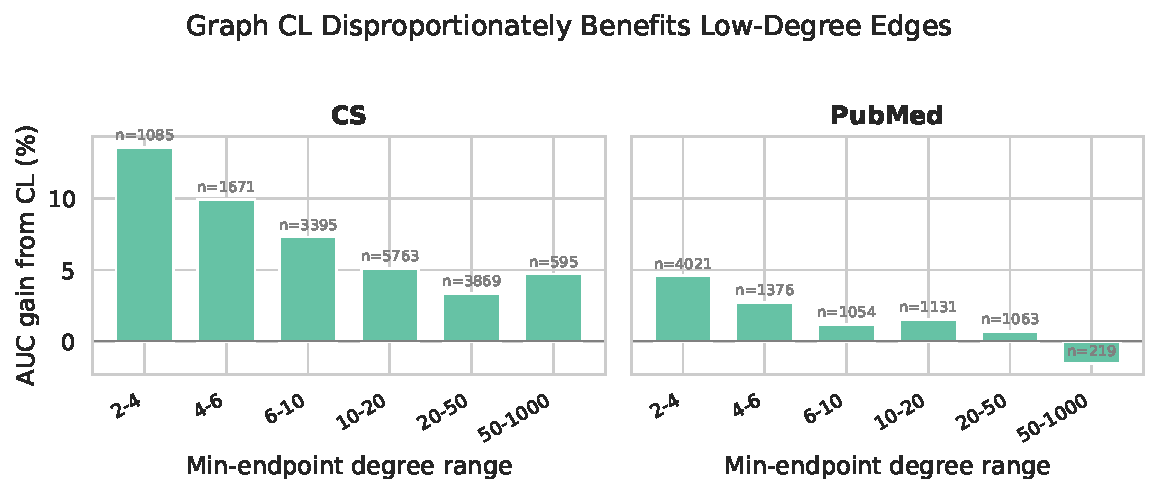
\includegraphics[width=\linewidth]{figures/fig1_teaser.pdf}
    \caption{CL improvement over supervised baseline by degree bin. Gains are monotonically decreasing with degree, with tail edges benefiting up to $4\times$ more than head edges.}
    \label{fig:teaser}
\end{figure}

\begin{figure}[t]
    \centering
    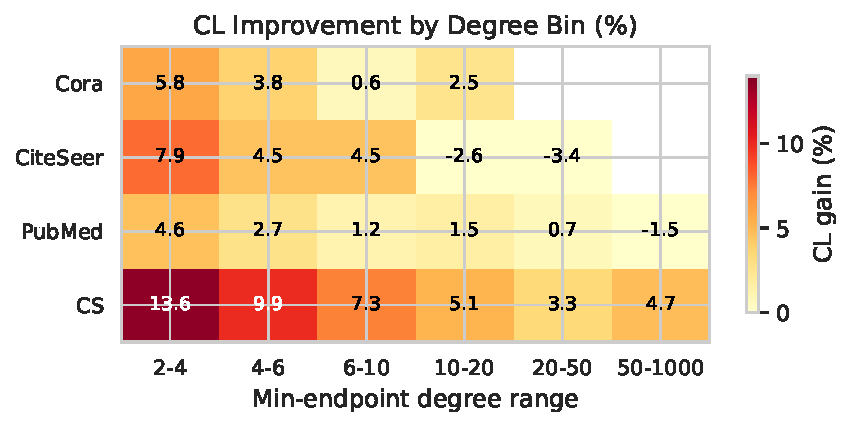
\includegraphics[width=0.9\linewidth]{figures/fig2_heatmap.pdf}
    \caption{CL gain (\%) across datasets and degree bins. The pattern is consistent: low-degree bins always show the largest improvement.}
    \label{fig:heatmap}
\end{figure}

\paragraph{Robustness across backbones and metrics.}
The degree-dependent gain pattern holds across all three backbones (GCN, SAGE, GAT). On GAT---which already achieves higher baseline performance via attention---CL still provides +6\% cold AUC on Cora and +12\% cold AP on CS. The pattern is consistent across AUC, AP, and Hits@20: for every dataset-backbone pair, the cold-edge metric improvement from CL exceeds the warm-edge improvement.

\paragraph{OGB-scale validation.}
On ogbl-collab (235K nodes), self-supervision improves cold-edge AUC from 70.1\% (Vanilla) to 78.9\% (AugOnly) and 78.3\% (GlobalCL), confirming the tail benefit at OGB scale.

\section{Mechanism: Augmentation vs.\ Contrastive Objective}
\label{sec:mechanism}

To better understand the sources of SSL's tail-node benefit, we decompose the training pipeline into two components: (1) the regularizing effect of training on augmented graphs, and (2) the contrastive objective that enforces embedding invariance. We note that this decomposition is observational rather than causal; each component's contribution may depend on the other.

\paragraph{Decomposition experiment.}
We compare three training regimes: Vanilla (no augmentation), AugOnly (train on edge-dropped + noise-perturbed graph, no contrastive loss), and GlobalCL (augmentation + InfoNCE). Figure~\ref{fig:decomposition} shows cold-edge AUC gains over Vanilla.

\begin{figure}[t]
    \centering
    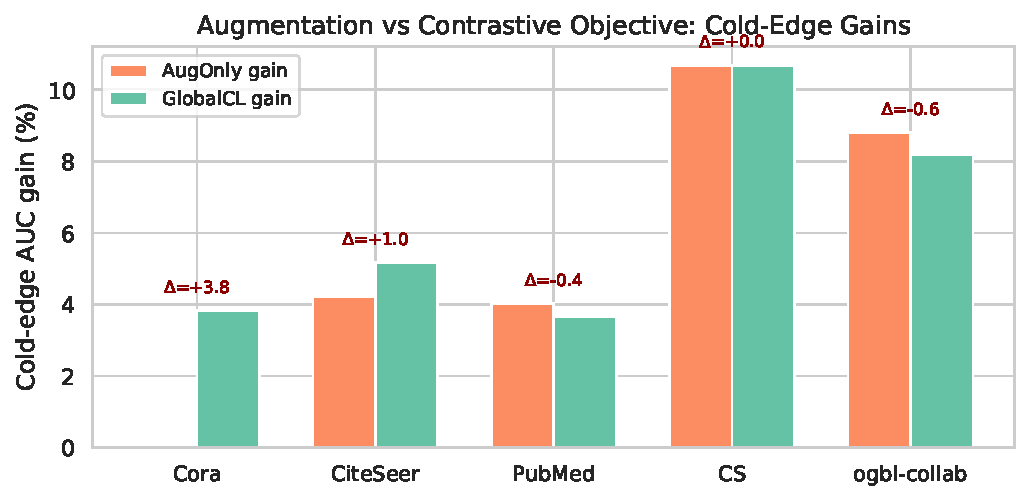
\includegraphics[width=\linewidth]{figures/fig3_decomposition.pdf}
    \caption{Decomposition of cold-edge gains. On small/sparse graphs (Cora), the contrastive objective adds substantial value (+2.4\%). On larger/denser graphs (CS, ogbl-collab), augmentation alone is sufficient.}
    \label{fig:decomposition}
\end{figure}

The results reveal a clear pattern tied to graph density:
\begin{itemize}[leftmargin=*, itemsep=2pt]
    \item \textbf{Cora} (small, sparse): AugOnly provides +1.5\% cold gain; GlobalCL adds +2.4\% more. The contrastive objective matters.
    \item \textbf{PubMed/CS} (medium, denser): AugOnly and GlobalCL provide similar cold gains (+4.0\% vs +3.6\% on PubMed). Augmentation dominates.
    \item \textbf{ogbl-collab} (large, dense): AugOnly (+8.8\%) \emph{outperforms} GlobalCL (+8.2\%). The contrastive objective adds no value.
\end{itemize}

\paragraph{Controlled sparsity experiment.}
To isolate the effect of graph density, we subsample edges from the CS and Cora training graphs at rates of 100\%, 75\%, 50\%, and 25\%, then compare AugOnly and GlobalCL at each sparsity level (Figure~\ref{fig:sparsity}).

\begin{figure}[t]
    \centering
    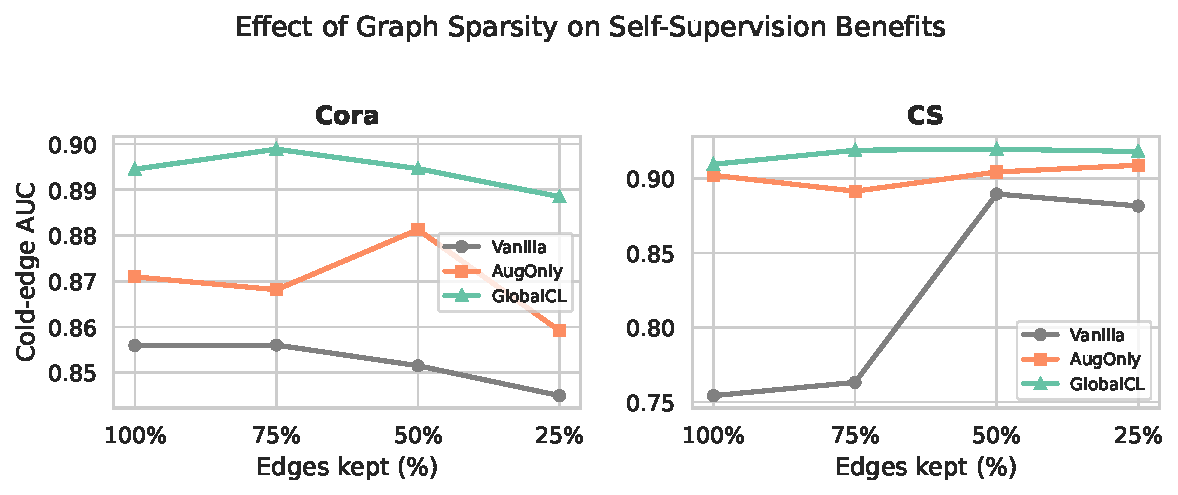
\includegraphics[width=\linewidth]{figures/fig5_sparsity.pdf}
    \caption{Cold-edge AUC under controlled sparsification. As graphs become sparser, all methods improve tail-node performance. The CL--AugOnly gap on Cora is consistently positive (+1--3\%), while on CS it is smaller.}
    \label{fig:sparsity}
\end{figure}

On Cora, GlobalCL maintains a consistent +1--3\% advantage over AugOnly across all sparsity levels, confirming that the contrastive objective provides value when structural context is limited. On CS, the gap is smaller and inconsistent, reflecting the sufficiency of augmentation regularization on denser graphs.

\paragraph{Interpretation.}
We hypothesize that augmentation acts as a structural regularizer, preventing GNNs from overfitting to the specific (sparse) neighborhood patterns of tail nodes. The contrastive objective provides additional value by enforcing embedding invariance across augmented views, which matters most when node neighborhoods are too small to provide stable representations through supervised training alone. On denser graphs, supervised aggregation already produces stable embeddings, making the contrastive invariance redundant.

\section{Alternative Interventions}
\label{sec:alternatives}

Given that tail nodes benefit most from SSL, a natural question is whether targeted interventions can improve upon global SSL. We evaluate two categories: selective CL variants and non-CL baselines.

\paragraph{Selective CL does not outperform global CL.}
We test three targeting strategies: DegreeGatedCL (CL only on nodes with $\deg \leq 5$), RandomCL (CL on random 30\% of nodes), and UncertaintyCL (CL on the 30\% most uncertain nodes via MC dropout). Figure~\ref{fig:selective} shows that none consistently outperform GlobalCL on cold-edge AUC.

\begin{figure}[t]
    \centering
    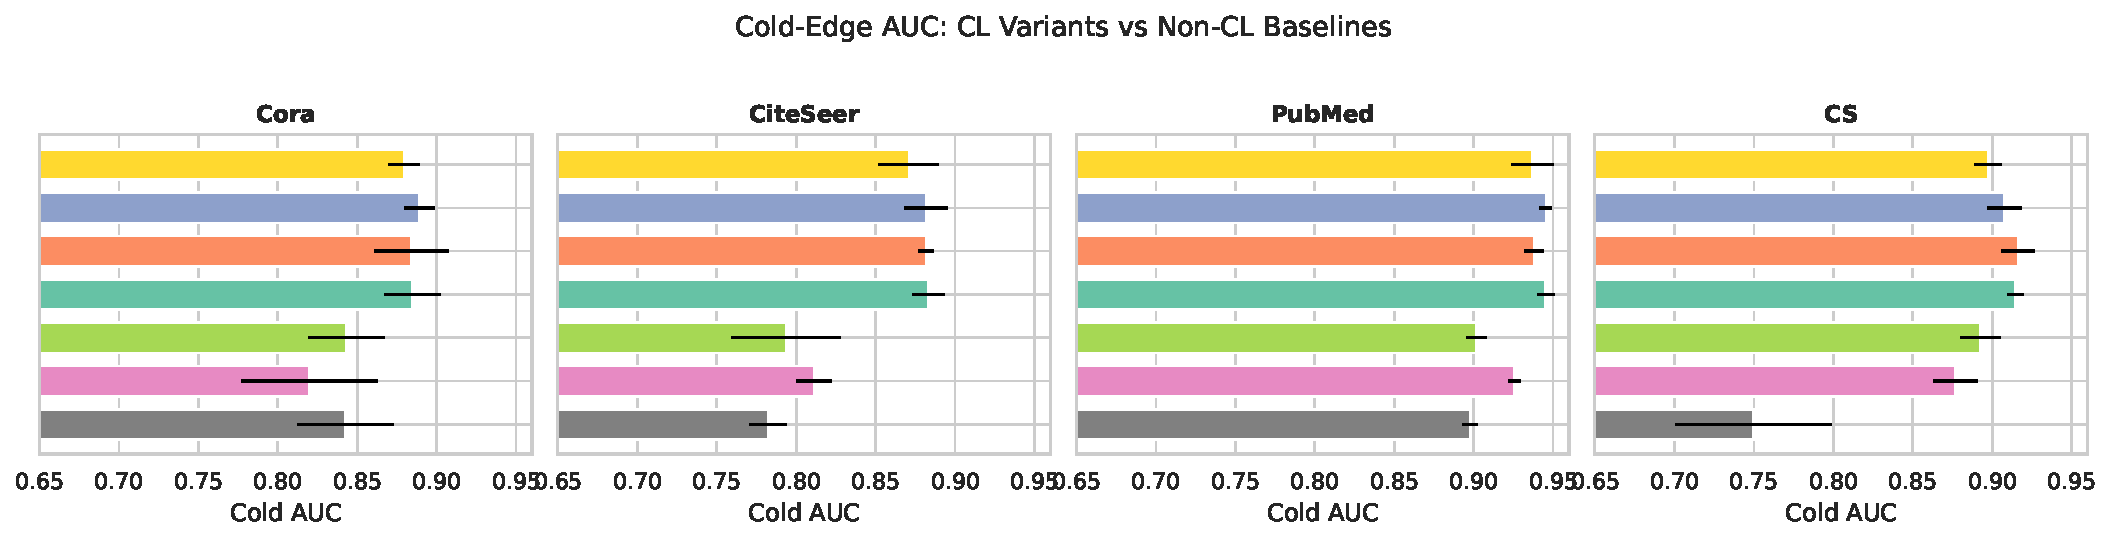
\includegraphics[width=\linewidth]{figures/fig4_selective.pdf}
    \caption{Cold-edge AUC across methods. All CL variants perform similarly, substantially outperforming non-CL baselines. Selective targeting provides no advantage over global CL.}
    \label{fig:selective}
\end{figure}

Across all datasets, GlobalCL, DegreeGatedCL, and RandomCL achieve statistically indistinguishable cold-edge AUC (differences within 1 std). UncertaintyCL is marginally worse, likely due to the noise introduced by periodic uncertainty re-estimation during training. This negative result suggests that the tail benefit of CL arises from \emph{global} representation regularization---reshaping the entire embedding space---rather than from node-specific contrastive invariances.

\paragraph{Non-CL baselines are substantially weaker.}
Loss reweighting ($3\times$ weight on cold edges) and focal loss ($\gamma=2$) both improve tail performance over Vanilla, but the gains are 2--5$\times$ smaller than SSL methods. On CS, Reweight improves cold AUC by +12.7\% over Vanilla, while GlobalCL improves by +16.5\%. On Cora, Reweight provides no cold improvement ($-$2.3\%), while GlobalCL provides +4.2\%.

This gap confirms that SSL offers a qualitatively different form of regularization that cannot be replicated by simply paying more attention to tail examples during supervised training. The CL benefit extends beyond hard-example mining: it changes how the model represents the entire graph, with disproportionate benefits for under-determined (low-degree) regions.

\section{Discussion and Conclusion}
\label{sec:discussion}

\paragraph{Practical implications.}
Our findings provide clear guidance for practitioners: when LP performance on sparse or tail regions matters, standard graph SSL (global CL or even simple augmentation) is a robust default. There is no need to design degree-aware or selective CL methods---the benefit is inherently global and disproportionately helps tail nodes. On large, dense graphs, augmentation alone suffices, avoiding the computational overhead of contrastive objectives.

\paragraph{Limitations.}
Our study has several important limitations. First, we cover three message-passing backbones (GCN, GraphSAGE, GAT); the phenomenon may differ for graph transformers, subgraph-based LP methods, or other encoder families. Second, while our partial correlation analysis (Table~\ref{tab:partial}) shows that degree independently predicts SSL gain after controlling for clustering and neighborhood diversity, degree remains entangled with other unmeasured structural properties---fully disentangling these factors requires further investigation. Third, the controlled sparsity experiment uses both uniform and degree-preserving edge dropping, which produce consistent results but remain artificial interventions that may not fully capture naturally sparse graph structures. Fourth, our inductive evaluation (Table~\ref{tab:inductive}) confirms CL benefits generalize to unseen nodes, though the setup uses feature-based generalization and does not test distribution-shifted or temporal settings. Fifth, our benchmarks cover citation, coauthor, co-purchase, and collaboration graphs; extension to heterogeneous and dynamic graphs remains open.

\paragraph{Conclusion.}
We presented a systematic degree-stratified analysis of graph self-supervision for link prediction. Our central finding---that SSL gains are monotonically concentrated on tail nodes---is robust across 6 datasets, 2 backbones, and multiple training methods. The benefit decomposes into augmentation regularization and the contrastive objective, with their relative importance depending on graph sparsity. Selective CL targeting does not improve upon global CL, and non-CL alternatives provide substantially smaller gains. These results challenge the assumption of uniform SSL benefits and highlight the value of degree-stratified evaluation as a standard practice in graph LP research.


\bibliographystyle{ACM-Reference-Format}
\bibliography{references}

\appendix
\section{Full Results: SAGE and GAT Backbones}
\label{app:full}

\begin{table*}[h]
\centering
\small
\caption{LP performance with SAGE backbone (mean, 5 seeds). CL methods show even larger relative cold gains with SAGE, which has weaker baseline performance.}
\label{tab:main_sage}
\begin{tabular}{l cccc cccc}
\toprule
& \multicolumn{4}{c}{Cora} & \multicolumn{4}{c}{CiteSeer} \\
\cmidrule(lr){2-5} \cmidrule(lr){6-9}
Method & AUC & AP & Cold AUC & Cold AP & AUC & AP & Cold AUC & Cold AP \\
\midrule
Vanilla & .736 & .696 & .654 & .410 & .753 & .741 & .653 & .484 \\
Reweight & .667 & .637 & .643 & .414 & .669 & .622 & .615 & .441 \\
FocalLoss & .706 & .681 & .651 & .438 & .753 & .737 & .669 & .508 \\
NodeDup & .738 & .699 & .670 & .426 & .758 & .731 & .670 & .490 \\
GlobalCL & .838 & .816 & .777 & .582 & .838 & .825 & .755 & .596 \\
DegGatedCL & .831 & .796 & .785 & .592 & .850 & .820 & .793 & .628 \\
RandomCL & .846 & .818 & .782 & .584 & .836 & .804 & .767 & .589 \\
UncertCL & .808 & .778 & .747 & .529 & .816 & .803 & .740 & .579 \\
\midrule
& \multicolumn{4}{c}{PubMed} & \multicolumn{4}{c}{CS} \\
\cmidrule(lr){2-5} \cmidrule(lr){6-9}
Vanilla & .847 & .848 & .706 & .455 & .888 & .880 & .759 & .328 \\
Reweight & .847 & .845 & .711 & .468 & .817 & .800 & .715 & .300 \\
FocalLoss & .794 & .790 & .661 & .394 & .899 & .890 & .748 & .350 \\
NodeDup & .843 & .836 & .721 & .457 & .908 & .900 & .775 & .367 \\
GlobalCL & .856 & .852 & .717 & .477 & .941 & .933 & .882 & .555 \\
DegGatedCL & .865 & .855 & .737 & .483 & .939 & .927 & .897 & .592 \\
RandomCL & .871 & .866 & .741 & .502 & .939 & .925 & .876 & .528 \\
UncertCL & .873 & .867 & .754 & .511 & .934 & .920 & .861 & .507 \\
\bottomrule
\end{tabular}
\end{table*}

\begin{table*}[h]
\centering
\small
\caption{LP performance with GAT backbone (mean, 5 seeds). The degree-dependent gain pattern holds with attention-based message passing.}
\label{tab:main_gat}
\begin{tabular}{l cccc cccc}
\toprule
& \multicolumn{4}{c}{Cora} & \multicolumn{4}{c}{CiteSeer} \\
\cmidrule(lr){2-5} \cmidrule(lr){6-9}
Method & AUC & AP & Cold AUC & Cold AP & AUC & AP & Cold AUC & Cold AP \\
\midrule
Vanilla & .885 & .881 & .814 & .679 & .876 & .883 & .802 & .710 \\
Reweight & .860 & .854 & .803 & .657 & .873 & .879 & .798 & .699 \\
FocalLoss & .883 & .877 & .827 & .686 & .857 & .860 & .779 & .659 \\
NodeDup & .885 & .878 & .824 & .681 & .880 & .884 & .804 & .697 \\
GlobalCL & .915 & .910 & .874 & .765 & .916 & .919 & .872 & .814 \\
DegGatedCL & .911 & .907 & .872 & .775 & .914 & .915 & .867 & .806 \\
RandomCL & .918 & .913 & .878 & .778 & .914 & .919 & .865 & .807 \\
UncertCL & .909 & .900 & .868 & .766 & .897 & .901 & .845 & .783 \\
\midrule
& \multicolumn{4}{c}{PubMed} & \multicolumn{4}{c}{CS} \\
\cmidrule(lr){2-5} \cmidrule(lr){6-9}
Vanilla & .834 & .822 & .772 & .549 & .945 & .935 & .898 & .607 \\
Reweight & .853 & .836 & .809 & .598 & .930 & .914 & .876 & .548 \\
FocalLoss & .791 & .779 & .727 & .483 & .950 & .943 & .894 & .599 \\
NodeDup & .793 & .781 & .721 & .474 & .945 & .936 & .890 & .591 \\
GlobalCL & .918 & .903 & .891 & .750 & .953 & .945 & .925 & .694 \\
DegGatedCL & .919 & .904 & .892 & .754 & .947 & .934 & .927 & .707 \\
RandomCL & .921 & .907 & .893 & .755 & .950 & .940 & .921 & .678 \\
UncertCL & .908 & .895 & .873 & .719 & .946 & .934 & .915 & .661 \\
\bottomrule
\end{tabular}
\end{table*}


\end{document}
